\documentclass[sigconf,review,anonymous]{acmart}

\usepackage{tikz}
\usetikzlibrary{positioning,arrows.meta,fit,backgrounds,calc}
\definecolor{cData}{RGB}{219,234,254}\definecolor{cDataB}{RGB}{37,99,235}
\definecolor{cFeat}{RGB}{220,252,231}\definecolor{cFeatB}{RGB}{22,163,74}
\definecolor{cModel}{RGB}{255,237,213}\definecolor{cModelB}{RGB}{234,88,12}
\definecolor{cEval}{RGB}{237,233,254}\definecolor{cEvalB}{RGB}{124,58,237}

\setlength{\textfloatsep}{7pt plus 2pt minus 2pt}
\setlength{\floatsep}{5pt plus 2pt minus 2pt}
\setlength{\intextsep}{6pt plus 2pt minus 2pt}
\setlength{\abovecaptionskip}{4pt}
\setlength{\belowcaptionskip}{2pt}
\setlength{\abovedisplayskip}{5pt plus 2pt minus 2pt}
\setlength{\belowdisplayskip}{5pt plus 2pt minus 2pt}
\setlength{\abovedisplayshortskip}{3pt plus 2pt minus 2pt}
\setlength{\belowdisplayshortskip}{3pt plus 2pt minus 2pt}

\AtBeginDocument{%
  \providecommand\BibTeX{{Bib\TeX}}}

\setcopyright{none}
\copyrightyear{2026}
\acmYear{2026}
\acmDOI{}
\acmConference[ICAIF '26]{ACM International Conference on AI in Finance}{November 14--17, 2026}{Milan, Italy}
\acmISBN{}

%% ============================================================================
%% v5 (THIS FILE is the canonical paper) -- language pass (2026-08-06) over the
%% v4 content: undergraduate-readable prose, conference register, no evaluative
%% adjectives; proofs unchanged; all numbers verbatim. The v4 files are frozen
%% at the pre-pass state; edit v5 only. _v5_1 is the named twin, regenerated
%% from v5, never edited directly.
%% v3/v4 -- full reposition for ICAIF '26 (deadline 2026-08-02 AoE).
%% NEW-MODEL SWITCH (2026-08-07): all model-dependent numbers now come from the
%% leak-free per-fold nested pipeline (coauthor reports in docs/rerun_2026-08-07/;
%% artifacts nested/perfect_pipeline_*.json and TP2MVTransformer/tables/
%% action_list/* on the compute side, committed there with stated gates).
%% LightGBM keeps its committed 149-feature fit (the F* selection never applied
%% to it), so its rows are unchanged. Unconditional and episode-classification
%% numbers are model-free and unchanged. Old-pipeline and new-pipeline numbers
%% must never mix (no-mixing rule); this file switched wholesale in one commit.
%%
%% REMAINING GAPS after the switch (fill only from new-model artifacts):
%% (a) 1.5x spread slippage was NOT rerun on the new models; every slippage
%%     claim was removed from the text. Restore only from a new-model artifact.
%% (b) win rate, mean trade return, skew (old Table 2 cols) and budget
%%     Sharpe/MaxDD/Calmar (old Table 3 cols) were not recomputed; the tables
%%     now report what the new artifacts support.
%% (c) per-model selected-tail calibration exists in newmodel_reruns.json;
%%     only the MLP values (0.695 / 37.7%) are quoted in text.
%% (d) no-history / permuted-history ablations were not rerun on the new
%%     pipeline; numeric ablation claims were removed.
%% (e) VERIFY[regime-mapping]: regime-concentration run-in maps R1 -> zero-
%%     premium regime, R3 -> positive-rate regime; confirm with coauthors.
%% (f) brief-25 decomposition N (234,885) vs the 250,004 candidate count is
%%     unreconciled; the text states shares and totals without that N.
%% (g) VERIFY[rev2-G] (price convention inside G) remains open.
%% (h) the half-sample Sharpe split (1.17 / 2.88) in the data section was an
%%     old-pipeline number; removed. Restore only from a new-model artifact.
%% DEADLINE 2026-08-09 AoE; the 8-page limit is the binding constraint.
%% ============================================================================

\begin{document}

\title{Machine-Learned Conditional Trading of TP2 Violations in SPY American Call Options}
\subtitle{From Near-Arbitrage Theory to Cost-Aware Selection}

\author{Anonymous Author(s)}
\affiliation{%
  \institution{Anonymous Institution}
  \country{}}

\renewcommand{\shortauthors}{Anonymous et al.}

\begin{abstract}
Total positivity of order two (TP2) imposes a restriction on European call prices across strikes and maturities: after the appropriate normalization, the price ratio of a higher-strike call to a lower-strike call should increase with maturity. This property holds in Black--Scholes and in a broader class of European option models~\cite{glasserman2026tp2theory}. Recent evidence further shows that TP2 violations in European SPX options can behave like near-arbitrage opportunities~\cite{glasserman2025tp2}. The same interpretation does not carry over directly to SPY. Its options are American, and early exercise around discrete dividends can itself produce an apparent TP2 violation.

We first ask when a violation in SPY calls can still be evaluated using the European TP2 benchmark. We derive two contract-level tests: a sufficient condition for the early-exercise premium to be zero and a dividend-based bound that identifies violations too large to be explained by early exercise. Among 177{,}487 detected episodes from 2014--2026, these tests resolve 64.0\% of the sample. In the 2021--2026 trading period, 71.0\% of episodes are European-equivalent under the zero-premium conditions.

We then ask whether TP2 violations are profitable after trading costs. Trading every detected candidate at quoted bid and ask prices wins 94.7\% of the time before commissions; adding them turns 250{,}004 trades into a \$12.52 million loss with a 12.9\% win rate. The signal survives the spread but not the commission charge, so we treat trading as a conditional selection problem. In six walk-forward test periods, LightGBM, an MLP, a TP2-specific transformer, and logistic regression all select subsets with positive aggregate out-of-sample P\&L. The MLP produces the largest normalized P\&L at \$3.47 million, while the transformer variants achieve active-day Sharpe ratios of 2.05 and 2.13, with date-clustered bootstrap intervals that exclude zero. In a separate premium-budget experiment, LightGBM and the MLP grow the budget by 14.6\% and 13.4\% per year. Overall, TP2 violations in SPY do not support unconditional trading after costs, but their profitability is concentrated in subsets that can be identified using information available when the violation occurs.
\end{abstract}

\begin{CCSXML}
<ccs2012>
 <concept>
  <concept_id>10010147.10010257.10010258.10010259</concept_id>
  <concept_desc>Computing methodologies~Machine learning</concept_desc>
  <concept_significance>500</concept_significance>
 </concept>
 <concept>
  <concept_id>10010405.10010481.10010485</concept_id>
  <concept_desc>Applied computing~Economics</concept_desc>
  <concept_significance>300</concept_significance>
 </concept>
</ccs2012>
\end{CCSXML}

\ccsdesc[500]{Computing methodologies~Machine learning}
\ccsdesc[300]{Applied computing~Economics}

\keywords{options trading, total positivity, American options, statistical arbitrage, machine learning, backtest validation, model selection}

\maketitle

\section{Introduction}
\label{sec:intro}

Option-pricing models can impose restrictions on the shape of the price surface that are stronger than no-arbitrage alone. Total positivity of order two (TP2) is one such restriction. For European calls, TP2 requires that, after the appropriate normalization, the price ratio of a higher-strike call to a lower-strike call increase with maturity. Glasserman and Pirjol show that this property holds in Black--Scholes and in a broader class of models characterized by mean-residual-life growth of the underlying distributions~\cite{glasserman2026tp2theory}. TP2 implies the usual calendar monotonicity of call prices, but the converse does not hold: an arbitrage-free model can violate TP2~\cite{glasserman2026tp2theory,glasserman2023convexity}. A TP2 violation is therefore not an arbitrage by definition. It is a failure of a stronger, testable restriction on the option-price surface.

For European SPX options, that distinction nevertheless has economic content. Glasserman, Li, and Pirjol find that TP2 violations are rare, tend to disappear within days, and support highly profitable trading strategies~\cite{glasserman2025tp2}. Their preferred T1 and K2 constructions win nearly every trade at mid-prices, and the T1 strategy remains profitable under a stronger quote-side screen that buys at the ask and sells at the bid. These results raise a natural question: does the same structure survive in SPY options, which provide exposure to the same index but trade as American-style options on a dividend-paying ETF?

American exercise changes the problem in an important way. For a European option, the observed price enters the TP2 inequality directly. For an American call, the observed value also contains an early-exercise premium, and that premium need not affect the four contracts in a TP2 rectangle symmetrically. Around discrete cash distributions, it can therefore create an apparent TP2 violation even when the corresponding European values do not violate the benchmark. We study calls because their early-exercise incentive is tied to these distributions; for American puts, interest on the strike creates an additional exercise incentive that is not confined to ex-dividend dates. The first question of the paper is thus not whether a detected SPY violation is profitable, but whether American exercise can explain it.

We give two computable answers. First, we derive sufficient conditions under which the early-exercise premium is zero, so the American call has the same frictionless value as its European counterpart (Proposition~\ref{prop:euro}). The condition holds when no ex-dividend date precedes expiry and, more generally, when the remaining distributions are small enough relative to the interest benefit from deferring payment of the strike. Second, when a positive early-exercise premium is possible, we derive a dividend-based certificate for violations that are too large to be explained by any admissible premium (Proposition~\ref{prop:cert}). Both tests can be evaluated contract by contract from announced distributions, interest rates, and market quotes. Among 177{,}487 detected SPY episodes from 2014--2026, the two tests resolve 64.0\% of the sample. During the 2021--2026 trading period, 71.0\% of episodes are European-equivalent under the zero-premium conditions.

The second question is whether these violations remain economically useful once they are traded rather than observed. We detect strong violations directly in NBBO bid and ask quotes, merge repeated signals into episodes, hold positions to expiration, and charge quoted spreads and commissions. Before commissions, SPY behaves like SPX: trading every candidate at the quoted bid and ask wins 94.7\% of the time and gains \$61.0M. After commissions, the same 250{,}004 trades over 2021--2026 lose \$12.52 million under our normalization, with a 12.9\% win rate and an active-day Sharpe ratio of $-1.01$. The violation signal is real, but on SPY it is not, by itself, a trading rule that survives costs.

This failure of unconditional trading turns the problem into one of conditional selection. Rather than search the entire option market for statistical patterns, we begin with a candidate set defined by economic theory and ask whether information available when the violation occurs can distinguish the small subset of trades that subsequently earn positive net returns. We formulate this as probabilistic classification and compare four model families with different inductive biases: LightGBM, a multilayer perceptron, an attention-based model designed for the TP2 episode structure, and logistic regression as a linear benchmark. Models are trained and evaluated chronologically in six walk-forward folds, calibrated on a separate validation year, and converted into trades using the same pre-specified probability rule. This design makes prediction, calibration, and realized cost-aware trading performance part of the same evaluation problem rather than treating classification accuracy as the endpoint.

Conditional selection changes the empirical result. Each model family selects a much smaller subset of violations and earns positive aggregate out-of-sample P\&L over the 2021--2026 test periods. The five-seed MLP ensemble earns \$3.47 million under the \$1{,}000-per-trade normalization, while the two transformer variants attain active-day Sharpe ratios of 2.05 and 2.13; the MLP and the ALiBi transformer are positive in all six test periods. Logistic regression also selects a profitable subset, showing that the result does not depend on a high-capacity architecture. Date-clustered bootstrap intervals are significantly positive for both transformer variants and for logistic regression, while the LightGBM and MLP totals are concentrated in fewer large winners. A separate premium-budget experiment produces a different ordering---LightGBM and the MLP grow the budget fastest, at 14.6\% and 13.4\% per year---highlighting the distinction between identifying profitable trades and allocating finite trading capital.

The paper therefore connects a structural restriction from option-pricing theory with a financial machine-learning decision problem. TP2 determines where to look; the American-option analysis determines when the European interpretation is defensible; and the learned models determine when a detected violation is worth trading after costs. The machine-learning task is consequently narrower than generic option-return prediction: every candidate is generated by the same theory-defined event, and the models are used only to condition the trading decision on information available at that event.

Our contributions are:
\begin{enumerate}
\item \textbf{An American-call interpretation of TP2 violations.}
For calls on an underlying with discrete cash distributions, we derive sufficient conditions for the early-exercise premium to be zero and a dividend-based certificate for violations that are too large for early exercise to explain (Propositions~\ref{prop:euro}--\ref{prop:cert}). The tests require only contract-level information available from announced distributions, interest rates, and quotes. Applied to the full SPY sample, they resolve 64.0\% of detected episodes and provide a theory-based explanation for why the European-equivalent share varies with the interest-rate regime.
\item \textbf{A cost-aware empirical benchmark for TP2 trading in SPY.}
We translate the SPX construction of~\cite{glasserman2025tp2} to American SPY calls while making the differences explicit: quote source, episode formation, forward adjustment under discrete distributions, expiration payoffs, and transaction costs. Strong violations are detected using executable quote sides, repeated observations are consolidated into episodes, and realized labels include quoted spreads and per-contract commissions. Under this construction, the unconditional strategy wins 94.7\% of trades before commissions yet is strongly unprofitable after them, locating the failure of the SPX near-arbitrage result on SPY in per-contract costs rather than in the violation signal.
\item \textbf{Theory-guided, walk-forward machine-learning selection.}
We formulate trading conditional on a detected TP2 violation as an out-of-sample classification problem and compare tree-based, feed-forward, attention-based, and linear models under a common chronological decision rule. Training, validation-year calibration, and testing are strictly separated in time, and the models are evaluated using both predictive metrics and realized portfolio outcomes. The selected subsets are profitable across all four model families, and robustness tests under clustered inference, trade exclusions, and finite premium budgets show where predictive performance does and does not translate into economically scalable performance.
\end{enumerate}

\section{TP2 Theory and the Trading Construction}
\label{sec:related}

\medskip\noindent\textbf{The TP2 Property of Call Prices.}
\label{sec:tp2theory}
Write $C(K,T)=\mathbb{E}[(S_T-K)^+]$ for the undiscounted European call value on a normalized underlying $\{S_t\}$ with $S_0=1$. Call prices are TP2 when, for all $K_1\le K_2$ and $T_1\le T_2$,
\begin{equation}
C(K_1,T_1)\,C(K_2,T_2)\;\ge\;C(K_1,T_2)\,C(K_2,T_1).
\label{eq:tp2}
\end{equation}
Equivalently, every $2\times2$ determinant $\det\left(\begin{smallmatrix} C(K_1,T_1) & C(K_1,T_2)\\ C(K_2,T_1) & C(K_2,T_2)\end{smallmatrix}\right)$ is non-negative, and the ratio $C(K_2,T)/C(K_1,T)$ increases with $T$. Glasserman and Pirjol establish this property for Black--Scholes calls at all strikes and characterize it, under regularity conditions, by growth of the underlying distributions in the mean-residual-life order~\cite{glasserman2026tp2theory}. TP2 implies calendar monotonicity but is not implied by no-arbitrage: arbitrage-free European models can fail TP2~\cite{glasserman2026tp2theory,glasserman2023convexity}. A market violation of Equation~\eqref{eq:tp2} is therefore a failure of the TP2 inequality for a four-contract rectangle, not by itself an arbitrage.

\medskip\noindent\textbf{The Forward-Adjusted Empirical Condition and the Four Trade Denominations.}
\label{sec:denominations}
With interest and dividends, the TP2 condition applies to strikes aligned in forward moneyness. Here $F_T$ is the parity-implied forward price, fitted cross-strike from put--call parity for each date and expiry, so market dividend expectations and rates enter the adjustment. For $T_1<T_2$ and $K_1/F_{T_1}<K_2/F_{T_2}$,
\begin{equation}
C(K_1,T_1)\,C(K_2,T_2)\;\ge\;C(\tilde K_1,T_2)\,C(\tilde K_2,T_1),
\label{eq:tp2adj}
\end{equation}
where $\tilde K_1=K_1 F_{T_2}/F_{T_1}$ and $\tilde K_2=K_2 F_{T_1}/F_{T_2}$, rounded up to traded strikes when needed~\cite{glasserman2025tp2}. The source transformation is derived by normalizing the dividend-paying asset by its forward price and assumes the normalized process satisfies the conditions of the European theory. Because SPY pays discrete cash distributions, we use the forward-adjusted inequality as an empirical benchmark rather than claim it as a theorem for SPY. Label the four contracts $A=C(K_1,T_1)$, $B=C(K_2,T_2)$, $C=C(\tilde K_1,T_2)$, $D=C(\tilde K_2,T_1)$, with superscripts $a$ and $b$ for ask and bid quotes. A \emph{violation} reverses Equation~\eqref{eq:tp2adj}; a \emph{strong violation} does so in quotes, $A^aB^a<C^bD^b$. This is conservative with respect to the quoted spread but does not by itself establish simultaneous execution at the displayed prices. The trading construction of~\cite{glasserman2025tp2} buys the undervalued pair and shorts the overvalued pair. Trades are grouped into four \emph{denominations} according to which two of the four contracts are traded; the entry prices of the two non-traded contracts serve as position weights, so the cash premium collected at entry equals the violation size for every denomination. For the two denominations we retain, writing $X^{w}$ for the weight given by the entry price of contract $X$, the expiration payoffs are
\[
\begin{aligned}
\Pi^{T_1} &= B^{w}\,(S_{T_1}-K_1)^+ - C^{w}\,(S_{T_1}-\tilde K_2)^+,\\
\Pi^{K_2} &= A^{w}\,(S_{T_2}-K_2)^+ - C^{w}\,(S_{T_1}-\tilde K_2)^+ .
\end{aligned}
\]
The $T_1$-denomination holds only near-expiry contracts; the $K_2$-denomination pairs the short near-dated $(\tilde K_2,T_1)$ leg with the long $(K_2,T_2)$ leg; the excluded $T_2$ and $K_1$ denominations short the longer-dated leg. The SPX study reports near-perfect hit rates for the T1 and K2 constructions at mid-prices, positive T1 results under its conservative strong-violation screen, and poor performance for the $T_2$ and $K_1$ denominations~\cite{glasserman2025tp2}. Our T1/K2 restriction (Section~\ref{sec:labels}) adopts this structure, and our four-denomination check reproduces the same asymmetry on SPY.

\medskip\noindent\textbf{From European Theory to American Practice: Two Reductions and a Certificate.}
\label{sec:american}
The TP2 theorems are proved for European-style, cash-settled options~\cite{glasserman2026tp2theory}. SPY calls are American-style on a dividend-paying ETF, so their values contain early-exercise premia $C^{\mathrm{am}}(K,T)=C^{\mathrm{eu}}(K,T)+\pi(K,T)$, $\pi(K,T)\ge0$, on both sides of Equation~\eqref{eq:tp2adj}~\cite{cosma2020earlyexercise}. At each signal date we take that date as time zero and assume deterministic cash distributions and discount factors, frictionless exercise, and no ownership benefit other than the stated distributions; the empirical classification approximates the discount curve with the contemporaneous three-month rate. The gap is smaller than it looks, and the three facts that close it have short proofs~\cite{merton1973,black1975}. (1)~Without dividends, a live call is worth at least its exercise value: $C^{\mathrm{eu}}_t\ge(S_t-Ke^{-r(T-t)})^+\ge(S_t-K)^+$ for $r\ge0$, so waiting is optimal and $C^{\mathrm{am}}=C^{\mathrm{eu}}$. (2)~With discrete dividends, the same bound applies on any interval containing no ex-dividend date, so early exercise can be optimal only immediately before an ex-date. (3)~The premium is bounded by the dividends: $\pi(K,T)\le\bar D(T):=\sum_{t_i\le T}\delta_i e^{-rt_i}$, their present value. To see this, take any exercise time $\tau$: the European lower bound $C^{\mathrm{eu}}_\tau\ge S_\tau-\mathrm{PV}_\tau(\text{dividends in }(\tau,T])-Ke^{-r(T-\tau)}$ gives $(S_\tau-K)^+\le C^{\mathrm{eu}}_\tau+\mathrm{PV}_\tau(\text{dividends in }(\tau,T])$; discounting to time 0, taking expectations, and optimizing over $\tau$ yields $C^{\mathrm{am}}\le C^{\mathrm{eu}}+\bar D(T)$, because the discounted European price is a martingale. These facts yield:

\begin{proposition}[Sufficient condition for zero early-exercise premium]\label{prop:euro}
If either (i) no ex-dividend date lies in $(0,T]$, or (ii) at every ex-date $t_i\le T$,
\begin{equation}
\textstyle\delta_i+\sum_{j>i,\,t_j\le T}\delta_j e^{-r(t_j-t_i)}\;\le\;K\big(1-e^{-r(T-t_i)}\big),
\label{eq:smalldiv}
\end{equation}
then $\pi(K,T)=0$: the frictionless American value coincides with its European counterpart. When the condition holds for all four contracts of a rectangle, the American early-exercise feature does not affect their frictionless values, and the rectangle can be evaluated against the European-call TP2 benchmark, subject to the assumptions on the normalized underlying and dividend adjustment used in the European theory~\cite{glasserman2026tp2theory}.
\end{proposition}
\begin{proof}
(i) is fact (1). For (ii): by fact (2), exercise can be optimal only at some ex-date $t_i$, where it is worth $(S_{t_i^-}-K)^+$. In states with $S_{t_i^-}\le K$ exercise is not optimal, so the comparison is needed only in the money. There, continuing is worth at least the value of holding to expiry, which the European lower bound puts at $S_{t_i^-}-\delta_i-\sum_{j>i,\,t_j\le T}\delta_je^{-r(t_j-t_i)}-Ke^{-r(T-t_i)}$. Continuation minus exercise is therefore at least the right side of \eqref{eq:smalldiv} minus its left side, which is non-negative. Exercise is never strictly better at any ex-date, so $\pi=0$.
\end{proof}
\noindent Condition (ii) applies the classical single-dividend bound behind Black's approximation~\cite{merton1973,black1975} at each ex-date in turn. Higher interest rates expand the set of dividend-spanning contracts satisfying the condition; whether it holds is contract-specific, depending on the strike, the dividend amounts, and the time from each ex-date to expiry (for $\delta_i/K=0.003$ the single-dividend break-even horizon is about 55 calendar days at $r=2\%$ and 22 at $r=5\%$). At $r\approx0$ (the 2021 regime) the condition fails for every contract spanning an ex-date. This gives a testable, theory-based account of regime dependence, separate from the label-rate shift documented in Section~\ref{sec:data}.

\begin{proposition}[Dividend-bound certificate]\label{prop:cert}
Let $\bar D_i=\bar D(T_i)$ and let $V^q:=C^bD^b-A^aB^a$ be the strong-violation size. If $V^q>M:=\bar D_2\,D^{b}+\bar D_1\,C^{b}$, and each NBBO brackets a frictionless American reference value ($C^{\mathrm{bid}}\le C^{\mathrm{am},*}\le C^{\mathrm{ask}}$ per contract), then the corresponding European values also violate Equation~\eqref{eq:tp2adj}: the American early-exercise premium cannot explain the observed inequality.
\end{proposition}
\begin{proof}
On the undervalued pair, $C^{\mathrm{eu}}\le C^{\mathrm{am},*}\le C^{\mathrm{ask}}$ bounds the European product above by $A^aB^a$. On each overvalued leg, $C^{\mathrm{eu}}\ge C^{\mathrm{am},*}-\bar D\ge C^{\mathrm{bid}}-\bar D$, and the condition ensures the relevant lower bounds are nonnegative before multiplication, giving $C^{\mathrm{eu}}(\tilde K_1,T_2)\,C^{\mathrm{eu}}(\tilde K_2,T_1)\ge C^bD^b-M$ (the cross term $\bar D_1\bar D_2\ge0$ only helps); chain the three inequalities.
\end{proof}
\noindent $M$ has the units of the price products; its economic size is best reported after normalization (for example $M/S_0^2$, or $M$ relative to the overvalued product), with each dividend term $\bar D_i$ of order $0.3$--$0.6\%$ of the underlying price and $\bar D_1=0$ when no ex-date precedes the near expiry. It can be computed per trade from announced dividends.

Each detected rectangle then falls into one of four categories: \emph{no-distribution European-equivalent} (no ex-date before $T_2$), \emph{dividend-spanning European-equivalent} (Proposition~\ref{prop:euro}(ii)), \emph{dividend-bound robust} (Proposition~\ref{prop:cert} among the remaining observations), and \emph{unresolved}. Because early-exercise premia enter both products, their nonnegativity alone does not determine the sign of the American-versus-European change; this is why the last category exists. Computed over all 177{,}487 episodes from announced dividends and the FRED three-month rate, 52.2\% span no distribution before $T_2$, 7.1\% satisfy the zero-premium dividend condition, 4.7\% satisfy the dividend-bound certificate, and 36.0\% remain unresolved.\footnote{The dividend-spanning European-equivalent share is zero through 2022 and 10--19\% in 2023--2025, tracking the short rate; the no-distribution share is calendar-driven. Per-year shares and the per-model classification of selected trades by category are part of the released implementation.} Over the 2021--2026 test span (125{,}002 episodes), the corresponding shares are 61.0\%, 10.0\%, 0.7\%, and 28.2\%, so 71.0\% of test-period episodes are European-equivalent under Proposition~\ref{prop:euro}. The learned selectors operate across all four categories. A full American-TP2 theorem remains open; one candidate route is to establish supermodularity of the optimal-stopping value in $(\log K,T)$ within the general lattice-theoretic framework of~\cite{topkis1998}.

The analysis is restricted to calls because the early-exercise mechanism is different for American puts. For calls, exercise pressure is tied to discrete distributions, which permits the dividend-based bounds above. For puts, the benefit from early exercise includes interest on the strike and can arise away from ex-dividend dates, so the reductions used here do not extend directly to American puts. This restriction concerns the American analysis in this paper; the European theory develops the corresponding RR2 property for puts, and the SPX study analyzes RR2 violations empirically~\cite{glasserman2026tp2theory,glasserman2025tp2}.
%% FIGURE-SLOT[regime] — SUSPENDED by review 2026-08-06 (one principal figure:
%% equity curves). figures/regime_partition.pdf remains committed for talks.
%% brief-15 remaining scope is covered by the regime-concentration run-in in
%% the Results robustness block (task-2.4 artifact), pending VERIFY[regime-mapping].

\medskip\noindent\textbf{Related Machine-Learning Work.}
ML for options spans surface fitting, hedging, pricing, and cross-sectional option-return prediction~\cite{bali2023option}, with an adjacent literature on ML for execution and market microstructure~\cite{kearns2013mlmicrostructure}; we pose the narrower problem of trade/no-trade classification conditional on a detected violation, scored by realized cost-aware performance. Boosting, deep, and linear models are all effective on the engineered episode features, with complementary strengths, in line with systematic tree-versus-neural comparisons on tabular data~\cite{grinsztajn2022why,gorishniy2021revisiting}. The transformer tests a multivariate ALiBi generalization~\cite{press2022alibi,shaw2018self} with five learned per-head distance slopes (Section~\ref{sec:transformer}). On evaluation, seed/budget sensitivity of ML comparisons~\cite{melis2018state,lucic2018gans,agarwal2021deep,bouthillier2021accounting,dodge2019show} and backtest multiple testing~\cite{white2000reality,harvey2016crosssection,bailey2014deflated} are established; we therefore fix the selection rules in advance and report seed-averaged ensembles.

\section{Data and Episode Construction}
\label{sec:data}

\medskip\noindent\textbf{Source, Scope, and a Regime Shift.}
\label{sec:data-source}
We use SPY American call options 2014--2026; the rolling evaluation trains from 2017 onward, the first year with enough episodes to form a training window. We exclude 2013 because its detected count (49{,}090 reported episodes versus 438 in 2014) is discontinuous with the subsequent sample: its violation rate is roughly thirty times the median of the other years and the excess is entirely in weekly expiries, a coverage anomaly of the feed rather than a market phenomenon. Quotes are the OPRA closing NBBO (Databento \texttt{OPRA.PILLAR}), taken as the last one-minute quote at or before 16:00~ET, with daily volume and open interest from the same feed. The panel covers the entire listed SPY chain each session, about 55--60M contract-session rows. The underlying close and realized distributions are the SPDR series. Mid prices, Black--Scholes implied volatilities inverted from the mid, spot delta, theta (per calendar day), and vega, and the parity-implied forward of Section~\ref{sec:denominations} are computed fields, not vendor data. Announced dividends and rates enter only the theory-side regime labels (Section~\ref{sec:american}). We require quotes for all four contracts of the rectangle, available adjusted strikes, and complete payoff and feature data; the resulting modeling universe is 177{,}487 unique episodes spanning 2014-02-03 to 2026-06-04, each contributing two candidate trades. Two facts matter downstream. First, episode frequency is highly non-stationary, rising by two orders of magnitude across the sample. Second, the profitable-label base rate $\pi_t$ collapses from 27--73\% in 2017--2020 to 11--16\% in 2021--2026: pair-weighted, the first four folds train at base rates of 39.9\%, 61.3\%, 46.8\%, and 43.4\% but test at 14.5--16.0\%, while the last two folds are nearly matched (15.4\%/15.6\% training versus 11.1\% test). The only pipeline component that adapts to this shift is a one-year isotonic calibration (Section~\ref{sec:calibration}).


\medskip\noindent\textbf{Episode Detection and Tracking.}
\label{sec:episode-tracking}
Our units are as follows: a \emph{daily violating pair} is a date-specific rectangle observation in the SPX study's sense; a \emph{rectangle} is the four contracts; an \emph{episode} merges consecutive daily observations of the same rectangle; a \emph{candidate trade} is an episode-denomination pair; a \emph{selected trade} is a candidate passing the selection policy. An episode begins when a rectangle is a strong violation, $A^aB^a<C^bD^b$ (Section~\ref{sec:denominations}), with the rounded-up adjusted strikes. The raw detector output is daily and rectangle-level. Treating each daily observation as an independent example would inflate the sample, so consecutive daily observations keyed on the near-leg contract are merged into one episode. This episode definition differs from the permanent-correction measure of the SPX study, which follows a fixed pair through its final violation date; ours is a sampling decision that avoids treating repeated signals as independent training examples. Over the full history, 2{,}430{,}220 daily observations collapse to 2{,}098{,}213 pair episodes with a median duration of one session (maximum 14). The 177{,}487-episode modeling universe is the downstream strong-violation, T1/K2, cost-labeled subset.

We also build a lifecycle panel following every episode over a fixed event-time window (20 pre-event sessions through expiration). The median normalized violation premium of Equation~\eqref{eq:tp2adj} is flat and slightly negative before the event, spikes at day 0 by construction, and decays toward zero over the following sessions, consistent with the fast reversion documented on SPX~\cite{glasserman2025tp2}. Although the panel runs through expiration, every lifecycle feature used as model input is truncated at event day 0; post-signal rows never enter the feature set.

\medskip\noindent\textbf{Labels, Costs, and the T1/K2 Restriction.}
\label{sec:labels}
The label policy holds positions to expiration and evaluates the payoffs $\Pi^{T_1}$ and $\Pi^{K_2}$ of Section~\ref{sec:denominations} from intrinsic value. This is the convention of the SPX study, whose violation trades are likewise held to expiry~\cite{glasserman2025tp2}, and it is the natural one here: 88.66\% of episodes are single-session, so most never present a distinct post-signal reversion exit, and a paired comparison on the selected trades finds hold-to-expiration ahead of an exit-at-reversion rule by \$3.94M in aggregate, so the expiry convention is not driving the results.
Entry executes at the quoted spread (buy at ask, sell at bid), with commissions of \$1.30 per contract per leg in total, charged as two \$0.65 sides, matching Interactive Brokers' published IBKR Lite rate per execution.\footnote{\url{https://www.interactivebrokers.com/en/pricing/commissions-options.php}, accessed 2026.} The normalized net profit of a candidate trade is
\[
R^{s}=\frac{\mathrm{premium}+\Pi^{s}-\mathrm{cost}^{s}}{G},\qquad s\in\{T_1,K_2\},
\]
where $G$ is the trade's gross entry exposure, the weighted sum of the two traded legs' entry prices.
%% VERIFY[rev2-G]: confirm the exact price convention in G (executed bid/ask vs
%% mid) from the label code and state it here in one clause.
Reported dollar P\&L equals $1000\,R^{s}$ per trade; it is a normalization, not the capital required to implement the trade (raw exposures range from a median of \$7--\$11 to \$814{,}000). Following the source construction, the backtest permits fractional contract quantities, with commissions charged proportionally. Terminal intrinsic-value accounting is a frictionless equivalent of expiration settlement: pin risk, exercise thresholds, assignment, stock delivery, and margin are not simulated, and the backtest does not credit interest on the initial premium or model financing. We restrict to the $T_1$- and $K_2$-denominations of Section~\ref{sec:denominations}, both of which short the shorter-dated $(\tilde K_2,T_1)$ leg. This is a structural prior fixed before any training, on two grounds. The excluded $T_2$/$K_1$ denominations short the longer-dated leg and so face a longer horizon for adverse moves, and the SPX study finds the same two denominations dominant per violation and per year~\cite{glasserman2025tp2}. The prior holds on SPY too: an unrestricted four-denomination LightGBM loses \$37.23M (Sharpe $-1.76$, 1/6 positive test periods), reproducing the SPX asymmetry in a different market, style, and cost regime.

\section{Models and Evaluation Protocol}
\label{sec:method}

For episode $i$ and denomination $s\in\{T_1,K_2\}$, define
\[
Y_{i,s}=\mathbf 1\{R^{\mathrm{net}}_{i,s}>0\},\qquad p_{i,s}=\Pr\big(Y_{i,s}=1\mid X_{i,s}\big),
\]
where $X_{i,s}$ collects the features below and $R^{\mathrm{net}}$ is the normalized net profit of Section~\ref{sec:labels}. For each episode, the denomination with the higher calibrated probability is traded if that probability is at least 0.5. The pipeline proceeds chronologically: detection, episode formation, feature construction, per-fold training, validation-year calibration, and test-year selection.


\medskip\noindent\textbf{Walk-Forward Design.}
We use six rolling folds covering test years 2021--2026: each trains on the three years ending two years before its test year, calibrates (isotonic) on the single intervening validation year, and evaluates once on the test year (so the first fold is 2017--2019 / 2020 / 2021 and the last is 2022--2024 / 2025 / 2026). Feature scaling is fit on training years only and calibration on the validation year only; no test-year information enters either. An expanding-window alternative is evaluated in Section~\ref{sec:robustness}.

\medskip\noindent\textbf{Feature Construction.}
\label{sec:features}
The contracts $A$--$D$ of Section~\ref{sec:denominations} give the naming convention: a feature prefixed $A$--$D$ is that quantity for that leg, and $D$ is the short near-dated leg. Per leg we record bid, ask, mid, quoted sizes, open interest, strike, calendar days to expiry, implied volatility, and delta, theta, and vega. Rectangle-level features are the mid-price violation size $C_{\mathrm{mid}}D_{\mathrm{mid}}-A_{\mathrm{mid}}B_{\mathrm{mid}}$ and its scale-free version, the strong-violation ratio $C^{b}D^{b}/(A^{a}B^{a})$, implied-volatility slopes and term spreads across legs and their average, the forwards and adjusted strikes, strike and maturity gaps, the underlying close, the traded pair's summed mid and mean relative spread, the signal month, and the pre-signal maximum of the normalized violation size. From a 149-candidate pool built from these quantities and their transforms, spanning eight semantic blocks, each fold selects its own 48-feature set $F^{\ast}_k$ from that fold's training years alone: five deterministic LightGBM~\cite{ke2017lightgbm} runs rank the pool by a blend of split-gain, split-count, and permutation importance, and the averaged ranking's top 48 are fixed before the calibration or test year is touched. Averaging over seeded runs removes borderline features that flip between runs, so each fold's selection is reproducible, and no calibration- or test-year information enters the feature choice. Per-feature definitions are documented in the released implementation.
$F^{\ast}_k$ contains no dividend or rate field: announced-dividend data carry look-ahead, so early-exercise pressure is inferred from the short leg's delta, theta, time to expiry, and moneyness. The MLP, the transformer, and the logistic regression use this identical per-fold 48-feature input. LightGBM is trained on the full 149-candidate pool and compared as a separate model family: the 48 features are LightGBM's own importance picks, so scoring it on them is a same-input control rather than a neutral comparison---restricting LightGBM to the selected features raises its Sharpe by 0.46---and the full pool is its natural configuration. Only feature \emph{values} feed the downstream models, so no model stacks on another. Architecture comparisons in Section~\ref{sec:results} are drawn among the models sharing the 48-feature input; comparisons involving LightGBM also reflect its different feature set.

\noindent\textbf{Implementation (all models).} Every model uses the six folds, per-fold feature selection (LightGBM excepted, as above), training-set standardization, validation-year isotonic calibration, and the $p\ge0.5$ rule. MLP and transformer results are five-seed ensembles: raw probabilities are averaged over the seeds before one calibration, because single-seed results vary materially with initialization; per-seed results are part of the released implementation. LightGBM and the logistic regression are single fits. LightGBM: 350 trees, learning rate 0.04, 31 leaves, balanced class weights. MLP (48-64-32-1, ReLU): Adam with $L_2$ regularization and early stopping. Transformer: hidden width 64, 4 heads, up to 64 history tokens, AdamW, validation-loss checkpointing, and a Huber auxiliary loss on realized return. An $L_2$-regularized logistic regression on $F^{\ast}_k$ serves as the logistic benchmark.

\medskip\noindent\textbf{The Transformer, Its Distance-Biased Variant, and Ablations.}
\label{sec:transformer}
Each candidate episode-strategy pair is a token combining its $F^{\ast}_k$ values, a strategy embedding, and calendar features. The token cross-attends to the 64 most recently dated episode tokens from strictly earlier calendar days---selected by date alone, never by label or outcome, zero-padded when fewer exist---with logits
$a^{h}_{ij}=q_i\!\cdot\!k_j/\sqrt{d}\,+\,\text{(same/cross-strategy bonus)}$.

\noindent\textbf{MV-ALiBi variant.} Generalizing ALiBi's scalar penalty~\cite{press2022alibi}, we subtract $m_h^{\top}d_{ij}$ from the logit, where $d_{ij}$ collects five domain distances between episodes $i,j$ and $m_h$ is a learned positive slope vector. The distance-biased variant edges plain attention (2.13 versus 2.05 with one additional positive test period, separated almost entirely by 2022; Table~\ref{tab:consolidated}), but the date-clustered interval on the difference includes zero, so we treat the gap as small and report both variants.

\medskip\noindent\textbf{Calibration and Trade Selection.}
\label{sec:calibration}
Isotonic regression~\cite{zadrozny2002transforming} is fit on validation-year predictions and applied unchanged to the subsequent test year. Ensembles average raw seed probabilities before calibration. All models use the pre-specified chronological rule of Section~\ref{sec:method}: a candidate trade is selected when its calibrated probability is at least 0.5. The same validation year is used for checkpoint selection and isotonic calibration; we note this as a limitation. Its residual effect is visible in the selected tail: the MLP's mean calibrated probability among selected trades is 0.695 while its selected win rate is 37.7\%, a temporal miscalibration the one-year isotonic fit does not remove; the transformers are the best calibrated of the five models on the pooled test population (Table~\ref{tab:calibration}).

\section{Results}
\label{sec:results}

All models are evaluated on the same walk-forward folds, with the same validation-year isotonic calibration and the same pre-specified chronological $p\ge0.5$ rule (one action per episode, ties broken toward T1); portfolio metrics are computed identically for every model. Active-day Sharpe annualizes ($\times\sqrt{252}$) the ratio of mean to standard deviation of daily P\&L over days with at least one open position; days without positions are omitted. We report total normalized P\&L, active-day Sharpe, a date-block bootstrap 95\% interval on total P\&L, and positive test periods. We supplement the flat-notional convention with an equal-weight premium-budget accounting experiment (Section~\ref{sec:capitalscaled}).

\medskip\noindent\textbf{Unconditional Baseline and the Consolidated Comparison.}
Trading all 250{,}004 candidate trades (two per episode) over 2021--2026 loses \$12.52M under the \$1{,}000 normalization (active-day Sharpe $-1.01$, max drawdown $-\$24.51$M, win rate 12.9\%, 2/6 positive test periods). The SPX study reports near-perfect hit rates for the same constructions at mid-prices and positive T1 results under its strong-violation screen~\cite{glasserman2025tp2}; under the SPY implementation studied here, the unconditional policy wins 12.9\% of the time. Where the loss comes from matters. At the quoted bid and ask prices alone, before commissions, the same trades win 94.7\% of the time and gain \$61.0M, hit rates comparable to the SPX study's; adding per-contract commissions produces the \$12.52M net loss. Under this construction the violation signal survives the spread. What it does not survive, at the \$1{,}000-per-trade normalization, is the commission charge---and the selection problem is to find the trades that clear it.
Each fitted model selects fewer trades than the unconditional policy and has positive aggregate normalized P\&L over the test periods (Table~\ref{tab:consolidated}, Figure~\ref{fig:equity}). The $L_2$ logistic regression earns \$1.35M at an active-day Sharpe of 1.82; the MLP ensemble has the largest total (\$3.47M); the ALiBi transformer has the highest Sharpe (2.13) and, with the MLP, positive P\&L in all six test periods. Date-block bootstrap 95\% intervals exclude zero for both transformer variants and the logistic regression, while the LightGBM and MLP intervals include zero: their totals are concentrated in fewer large winners. Random selection does not explain the gains: 1{,}000 draws matched to each model's trade count lose \$0.71M on average, and draws additionally matched to each model's active days and daily trade counts exceed the plain transformer's total in only 8\% of draws. LightGBM is the exception under that day-matched comparison (67\% of draws exceed it), so its edge lies mainly in day selection.

\begin{figure}[t]
\centering
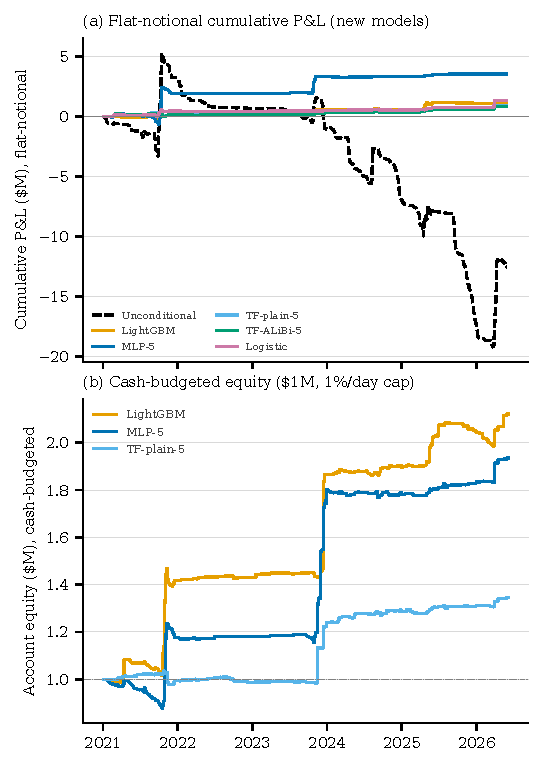
\includegraphics[width=\linewidth]{figures/equity_curves_newmodel.pdf}
\caption{Test periods 2021--2026. (a)~Cumulative normalized P\&L under the \$1{,}000-per-trade convention: the unconditional policy (dashed) loses \$12.52M; every model-selected subset ends positive. (b)~Account equity in the premium-budget accounting experiment (\$1M start, 1\%-of-cash daily cap) for LightGBM, the MLP, and the plain transformer.}
\label{fig:equity}
\end{figure}

\begin{table}[t]
\centering
\footnotesize
\resizebox{\linewidth}{!}{%
\begin{tabular}{lrrrcc}
\toprule
Method & Trades & Total P\&L & Active-day Sharpe & 95\% CI on P\&L & Pos.\ periods \\
\midrule
Unconditional & 250{,}004 & $-$\$12.52M & $-$1.01 & --- & 2/6 \\
LightGBM & 19{,}636 & \$682K & 1.25 & $[-\$0.14\mathrm{M},\ \$1.61\mathrm{M}]$ & 5/6 \\
MLP (5-seed) & 19{,}398 & \$3.47M & 1.92 & $[-\$0.77\mathrm{M},\ \$10.11\mathrm{M}]$ & 6/6 \\
Transformer (plain, 5-seed) & 15{,}931 & \$840K & 2.05 & $[\$0.06\mathrm{M},\ \$1.41\mathrm{M}]$ & 5/6 \\
Transformer (ALiBi, 5-seed) & 15{,}542 & \$866K & 2.13 & $[\$0.07\mathrm{M},\ \$1.47\mathrm{M}]$ & 6/6 \\
Logistic ($L_2$) & 12{,}803 & \$1.35M & 1.82 & $[\$0.05\mathrm{M},\ \$2.73\mathrm{M}]$ & 5/6 \\
\bottomrule
\end{tabular}%
}
\caption{Consolidated comparison over the 2021--2026 test periods (2026 is partial). All models use per-fold nested feature selection (LightGBM: full 149-feature pool), validation-year isotonic calibration, and the pre-specified $p\ge0.5$ one-action rule. MLP and transformer rows are five-seed ensembles (raw probabilities averaged before one calibration); LightGBM and the logistic regression are single fits. The 95\% interval is a date-block bootstrap on total P\&L; dollar figures under the \$1{,}000-per-trade normalization.}
\label{tab:consolidated}
\end{table}

%% NOTE (PI decision 2026-08-05): the operating-point-confound contribution,
%% seed-dispersion discussion, matched-selectivity run-in, and selectivity
%% figure were removed in full. Do not reintroduce them. The committed artifacts
%% (selectivity_sweep.csv, mlp5_sweep_verdict.json, DSR JSONs, figure) remain
%% the internal record. Table 2 reports the five-seed protocol only.

\medskip\noindent\textbf{Equal-Weight Premium-Budget Accounting Experiment.}
\label{sec:capitalscaled}
The \$1{,}000-per-trade normalization isolates selection quality but assumes unlimited capital. We also track a cash balance: \$1M starting cash, at most 1\% of available cash committed to new-position premium each day, equal weighting within a day. This calculation differs from the gross-exposure sizing rule of the SPX study~\cite{glasserman2025tp2}, so its output is a normalized cash-balance growth rate, not a deployable return on capital. LightGBM and the MLP grow the budget fastest (14.6\% and 13.4\% per year); the transformers and the logistic regression grow it at 6--7\% (Table~\ref{tab:capitalscaled}, Figure~\ref{fig:equity}b). The level is sensitive to sizing: integer contract quantities move growth by model-dependent amounts in both directions, and reserving Reg-T margin for the short legs---a conservative, no-netting model---compresses growth to 1--2\% per year for every model. The differences between Table~\ref{tab:consolidated} and Table~\ref{tab:capitalscaled} separate identifying profitable trades from allocating finite capital to them.

\begin{table}[t]
\centering
\footnotesize
\begin{tabular}{lrrr}
\toprule
Model & Premium & Integer & Reg-T margin \\
\midrule
Unconditional & $-11.7\%$ & --- & --- \\
LightGBM & 14.6\% & 11.0\% & 1.0\% \\
MLP (5-seed) & 13.4\% & 7.2\% & 1.3\% \\
Transformer (plain, 5-seed) & 6.7\% & 3.3\% & 2.2\% \\
Transformer (ALiBi, 5-seed) & 6.1\% & 8.1\% & 2.3\% \\
Logistic ($L_2$) & 7.4\% & 31.5\% & 1.9\% \\
\bottomrule
\end{tabular}
\caption{Annualized growth in the equal-weight premium-budget accounting experiment, 2021--2026 (\$1M starting cash, 1\%-of-cash daily premium cap, equal weighting within a day), under three sizing conventions: fractional contracts (baseline), integer contracts (rounded, minimum one), and fractional with Reg-T margin reserved for the short legs (conservative, no netting). A normalization of cash-balance growth, not deployable return on capital.}
\label{tab:capitalscaled}
\end{table}

\medskip\noindent\textbf{Robustness.}
\label{sec:robustness}

\noindent\textbf{Strategy-level breakdown.} By denomination, the MLP ensemble earns \$0.99M on T1 and \$2.48M on K2, both positive; LightGBM is the most balanced (T1 \$378K at Sharpe 0.85, K2 \$304K at 1.74). Neither model's total rests on a single denomination.

\noindent\textbf{By test period.} Unconditional trading loses in four of six test periods, with swings one to two orders of magnitude larger than any learned model's; the learned models remain in a narrow, mostly positive band (Figure~\ref{fig:equity}a). The MLP and the ALiBi transformer are positive in all six periods; the plain transformer and the logistic regression are negative only in 2022 ($-\$27$K and $-\$34$K), where the ALiBi variant holds at $+\$3$K; LightGBM has one negative period.

\noindent\textbf{Excluding the partial year.} 2026 covers $\approx$107 trading days; re-running the unconditional baseline on 2021--2025 strengthens the contrast ($-\$17.45$M, Sharpe $-1.73$).

\noindent\textbf{Training window.} For LightGBM, an expanding window earns more raw dollars (\$734.9K vs.\ \$686.2K) from higher late-sample volume at lower quality, but loses on Sharpe in five of six years with the only negative year (2024, $-0.13$ vs.\ 1.59); we keep the three-year window.

\noindent\textbf{Early assignment.} Trades whose short leg spans an ex-dividend date (early-assignment risk the expiry labels do not price) are 16--27\% of selections. Excluding them raises the Sharpe of LightGBM (1.25 to 1.42), the MLP (1.92 to 2.19), and the logistic regression (1.82 to 1.93) and slightly lowers the transformers' (2.05 to 1.88, 2.13 to 2.02); every model remains profitable, so short-leg dividend exposure does not carry the results.

\noindent\textbf{Selection rule.} Replacing the pre-specified $p\ge0.5$ rule with a value rule that trades whenever the predicted expected normalized return is positive raises LightGBM's total P\&L to \$3.80M but lowers its active-day Sharpe to 0.94: the value rule admits many marginal trades. We retain the probability rule.

\noindent\textbf{Quote quality and the forward.} Individually, stricter quote-quality screens leave the results intact; imposing all of them jointly retains only 5--7\% of candidates and eliminates the aggregate profitability, so the strategies depend on typical quotes rather than on a small, unusually clean subset. Re-detecting violations under an independently estimated forward keeps 66\% of episodes' adjusted-strike targets and leaves the sign of every model's aggregate P\&L unchanged.

\noindent\textbf{Regime concentration.} Split by the dividend--rate regime of the episode date, the MLP and the logistic regression earn 93--95\% of their totals on episodes in the zero-premium regime, where the European reading is direct; the transformers earn roughly half of theirs (53--54\%) in the later positive-rate regime, where early exercise is live.
%% VERIFY[regime-mapping]: confirm with coauthors that R1 = zero-premium regime
%% and R3 = positive-rate regime in the task-2.4 artifact before submission.

\noindent\textbf{Feature-selection stability.} Re-running the per-fold selection with three independent seed sets gives an MLP Sharpe of $2.16\pm0.38$: the reported figures reflect the method, not one selection draw.

\noindent\textbf{Market exposure.} Returns retain positive SPY exposure despite predominantly net-short entry delta (82\% of trades, a structural consequence of shorting the near leg). For the MLP, a trade-level regression of returns on the underlying's move gives a beta of 16.5 that falls to 8.3 once a squared-move term is added: much of the exposure is short-gamma path dependence from the short near-dated leg rather than directional positioning. The strategies should not be described as market-neutral.

\noindent\textbf{Classification metrics.} On the pooled test population (base rate $\approx$13.8\%, identical across models by construction), Table~\ref{tab:calibration} reports the Brier score and expected calibration error. The transformers are the best calibrated (ECE 0.036--0.038) and the MLP the least (0.065), consistent with its selected-tail miscalibration (Section~\ref{sec:calibration}); calibration quality does not order P\&L, since the MLP holds the largest total with the weakest calibration.

\begin{table}[t]
\centering
\footnotesize
\begin{tabular}{lrr}
\toprule
Model & Brier & ECE \\
\midrule
LightGBM & 0.086 & 0.049 \\
MLP (5-seed) & 0.113 & 0.065 \\
Transformer (plain, 5-seed) & 0.087 & 0.036 \\
Transformer (ALiBi, 5-seed) & 0.087 & 0.038 \\
Logistic ($L_2$) & 0.093 & 0.049 \\
\bottomrule
\end{tabular}
\caption{Brier score and expected calibration error (10 equal-width bins) on the pooled 2021--2026 test population (base rate $\approx$13.8\%).}
\label{tab:calibration}
\end{table}

\section{Discussion and Threats to Validity}
\label{sec:limitations}

\noindent\textbf{What is established.} Under the stated assumptions, part of the sample has zero early-exercise premium (59.3\% across the two European-equivalent categories), and the dividend bounds classify a further 4.7\%. Under the paper's quote, payoff, and cost construction, unconditional trading has negative aggregate normalized P\&L, and each classifier-selected subset has positive aggregate normalized P\&L over the test periods. Most of the performance comes from the episode construction and the feature set: even the logistic benchmark is profitable, with a date-clustered interval that excludes zero. The largest total (the MLP's) is concentrated in a few large winners and its interval includes zero, while the transformer and logistic totals are smaller but significantly positive.

\noindent\textbf{What is not identified.} Within SPY, the decomposition of Section~\ref{sec:results} attributes the unconditional reversal to commissions under the stated normalization. Across markets, the comparison with the SPX study still changes the underlying, settlement, the sample period, the quote source, and the episode construction together, so cross-market differences are not attributed to a single cause. The classification of episodes by Propositions~\ref{prop:euro}--\ref{prop:cert} bounds what early exercise can explain; it does not establish that every European-equivalent rectangle must satisfy TP2.

\noindent\textbf{Implementation limitations.} Assignment is not simulated, and 16--27\% of selected trades carry short-leg ex-dividend timing; quantities are fractional in the baseline, and reserving Reg-T margin compresses premium-budget growth to 1--2\% per year; the forward adjustment is an empirical benchmark under discrete distributions; returns carry positive directional exposure; the base rate shifts $\sim$4$\times$ between the early training folds and the test periods, absorbed only by the one-year isotonic fit; and $F^{\ast}_k$ has no scale-invariant price-ratio feature while the underlying drifts 50--80\% across the sample. All code and derived episode/feature/label datasets will be released on acceptance; the raw vendor quote feed cannot be redistributed.

\section{Conclusion}
Recent European-option theory identifies TP2 as a restriction on call prices across strike and maturity. The restriction is stronger than calendar monotonicity and is not a general consequence of no-arbitrage. Its application to SPY calls is complicated by American exercise and discrete ETF distributions. We give sufficient conditions under which an American call has no early-exercise premium and a dividend-based condition under which the available premium bounds cannot explain a strong quote-side violation. These results classify what the American exercise feature can explain; they do not establish that every European-equivalent rectangle must satisfy TP2.

Under the SPY quote, payoff, and cost construction used here, the violations win almost every trade before commissions, yet unconditional trading has negative aggregate normalized P\&L after them; walk-forward classifiers select smaller subsets whose aggregate normalized P\&L remains positive across all four model families.

\bibliographystyle{ACM-Reference-Format}
\begingroup
\footnotesize
\setlength{\itemsep}{0pt}
\setlength{\parskip}{0pt}
\begin{thebibliography}{27}

\bibitem{glasserman2025tp2}
Paul Glasserman, Mike Li, and Dan Pirjol. 2025. Trading TP\textsubscript{2} Option Violations. \textit{Quantitative Finance} 25, 8 (2025), 1177--1198. \url{https://doi.org/10.1080/14697688.2025.2538597}

\bibitem{press2022alibi}
Ofir Press, Noah A. Smith, and Mike Lewis. 2022. Train Short, Test Long: Attention with Linear Biases Enables Input Length Extrapolation. In \textit{International Conference on Learning Representations (ICLR)}.

\bibitem{glasserman2026tp2theory}
Paul Glasserman and Dan Pirjol. 2026. When Are Option Prices TP\textsubscript{2}? \textit{Mathematical Finance} 36, 3 (2026), 571--594. \url{https://doi.org/10.1111/mafi.70024}

\bibitem{glasserman2023convexity}
Paul Glasserman and Dan Pirjol. 2023. Total Positivity and Relative Convexity of Option Prices. \textit{Frontiers of Mathematical Finance} 2, 1 (2023), 1--32. \url{https://doi.org/10.3934/fmf.2023001}

\bibitem{merton1973}
Robert C. Merton. 1973. Theory of Rational Option Pricing. \textit{Bell Journal of Economics and Management Science} 4, 1 (1973), 141--183. \url{https://doi.org/10.2307/3003143}

\bibitem{black1975}
Fischer Black. 1975. Fact and Fantasy in the Use of Options. \textit{Financial Analysts Journal} 31, 4 (1975), 36--41, 61--72. \url{https://doi.org/10.2469/faj.v31.n4.36}

\bibitem{topkis1998}
Donald M. Topkis. 1998. \textit{Supermodularity and Complementarity}. Princeton University Press.

\bibitem{ke2017lightgbm}
Guolin Ke et al. 2017. LightGBM: A Highly Efficient Gradient Boosting Decision Tree. In \textit{NeurIPS 30}, 3146--3154.

\bibitem{zadrozny2002transforming}
Bianca Zadrozny and Charles Elkan. 2002. Transforming Classifier Scores into Accurate Multiclass Probability Estimates. In \textit{KDD}, 694--699. \url{https://doi.org/10.1145/775047.775151}

\bibitem{cosma2020earlyexercise}
Antonio Cosma et al. 2020. Early Exercise Decision in American Options with Dividends, Stochastic Volatility, and Jumps. \textit{J.\ Financial and Quantitative Analysis} 55, 1 (2020), 331--356. \url{https://doi.org/10.1017/S0022109018001229}

\bibitem{kearns2013mlmicrostructure}
Michael Kearns and Yuriy Nevmyvaka. 2013. Machine Learning for Market Microstructure and High Frequency Trading. In \textit{High-Frequency Trading}. Risk Books.

\bibitem{kunsch1989}
Hans R. K\"unsch. 1989. The Jackknife and the Bootstrap for General Stationary Observations. \textit{Annals of Statistics} 17, 3 (1989), 1217--1241. \url{https://doi.org/10.1214/aos/1176347265}

\bibitem{bailey2014deflated}
David H. Bailey and Marcos L\'opez de Prado. 2014. The Deflated Sharpe Ratio: Correcting for Selection Bias, Backtest Overfitting, and Non-Normality. \textit{Journal of Portfolio Management} 40, 5 (2014), 94--107. \url{https://doi.org/10.3905/jpm.2014.40.5.094}

\bibitem{harvey2016crosssection}
Campbell R. Harvey, Yan Liu, and Heqing Zhu. 2016. $\ldots$ and the Cross-Section of Expected Returns. \textit{Rev.\ Financial Studies} 29, 1 (2016), 5--68. \url{https://doi.org/10.1093/rfs/hhv059}

\bibitem{white2000reality}
Halbert White. 2000. A Reality Check for Data Snooping. \textit{Econometrica} 68, 5 (2000), 1097--1126. \url{https://doi.org/10.1111/1468-0262.00152}

\bibitem{bouthillier2021accounting}
Xavier Bouthillier et al. 2021. Accounting for Variance in Machine Learning Benchmarks. In \textit{MLSys} 3.

\bibitem{dodge2019show}
Jesse Dodge et al. 2019. Show Your Work: Improved Reporting of Experimental Results. In \textit{EMNLP-IJCNLP}, 2185--2194. \url{https://doi.org/10.18653/v1/D19-1224}

\bibitem{melis2018state}
G\'abor Melis, Chris Dyer, and Phil Blunsom. 2018. On the State of the Art of Evaluation in Neural Language Models. In \textit{International Conference on Learning Representations (ICLR)}.

\bibitem{lucic2018gans}
Mario Lucic et al. 2018. Are GANs Created Equal? A Large-Scale Study. In \textit{NeurIPS 31}, 698--707.

\bibitem{agarwal2021deep}
Rishabh Agarwal et al. 2021. Deep Reinforcement Learning at the Edge of the Statistical Precipice. In \textit{NeurIPS 34}, 29304--29320.

\bibitem{grinsztajn2022why}
L\'eo Grinsztajn, Edouard Oyallon, and Ga\"el Varoquaux. 2022. Why Do Tree-Based Models Still Outperform Deep Learning on Typical Tabular Data? In \textit{NeurIPS 35 D\&B}. \url{https://doi.org/10.52202/068431-0037}

\bibitem{gorishniy2021revisiting}
Yury Gorishniy et al. 2021. Revisiting Deep Learning Models for Tabular Data. In \textit{NeurIPS 34}, 18932--18943.

\bibitem{shaw2018self}
Peter Shaw, Jakob Uszkoreit, and Ashish Vaswani. 2018. Self-Attention with Relative Position Representations. In \textit{NAACL-HLT}, 464--468. \url{https://doi.org/10.18653/v1/N18-2074}

\bibitem{bali2023option}
Turan G. Bali et al. 2023. Option Return Predictability with Machine Learning and Big Data. \textit{Rev.\ Financial Studies} 36, 9 (2023), 3548--3602. \url{https://doi.org/10.1093/rfs/hhad017}

\end{thebibliography}
\endgroup

\end{document}
